%% LaTeX-Beamer template for KIT design
%% by Erik Burger, Christian Hammer
%% title picture by Mathias.Landhaeusser@kit.edu

\documentclass[18pt]{beamer}

%% SLIDE FORMAT

% use 'beamerthemekit' for standard 4:3 ratio
% for widescreen slides (16:9), use 'beamerthemekitwide' and change titleimage to 'Folientitelbild_wide'

\usepackage{templates/beamerthemekit}
%\usepackage{templates/beamerthemekitwide}

%% TITLE PICTURE

% if a custom picture is to be used on the title page, copy it into the 'logos'
% directory, in the line below, replace 'mypicture' with the 
% filename (without extension) and uncomment the following line
% (picture proportions: 63 : 20 for standard, 169 : 40 for wide
% *.eps format if you use latex+dvips+ps2pdf, 
% *.jpg/*.png/*.pdf if you use pdflatex)

%\titleimage{Folientitelbild_wide}

%% TITLE LOGO

% for a custom logo on the front page, copy your file into the 'logos'
% directory, insert the filename in the line below and uncomment it

%\titlelogo{infofak}

% (*.eps format if you use latex+dvips+ps2pdf,
% *.jpg/*.png/*.pdf if you use pdflatex)

%% TikZ INTEGRATION

% use these packages for PCM symbols and UML classes
% \usepackage{templates/tikzkit}
% \usepackage{templates/tikzuml}

% the presentation starts here

\title[Maschinelles Lernen]{Maschinelles Lernen im Kontext der Programmierung in natürlicher Sprache}
\subtitle{Betreut von Alexander Wachtel}
\author{Philipp Weinmann}

\institute{IPD Tichy}

% Bibliography

\usepackage[citestyle=numeric,bibstyle=numeric,hyperref,backend=bibtex,citestyle=alphabetic,bibstyle=authoryear]{biblatex}
\bibliography{Abschlussvortrag.bib}
\bibhang1em

\begin{document}

% change the following line to "ngerman" for German style date and logos
\selectlanguage{ngerman}

%title page
\begin{frame}
\titlepage
\end{frame}

%table of contents
\begin{frame}{Outline/Gliederung}
\tableofcontents
\end{frame}

%%BEGIN

\section{Einordnung von maschinellem Lernen}

\begin{frame}{Einleitung}
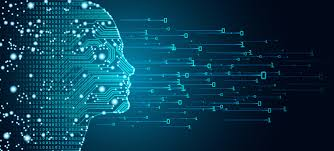
\includegraphics{images/Hype.jpg}
\cite{Hype}
\end{frame}

\begin{frame}{Einordnung von maschinellem Lernen}
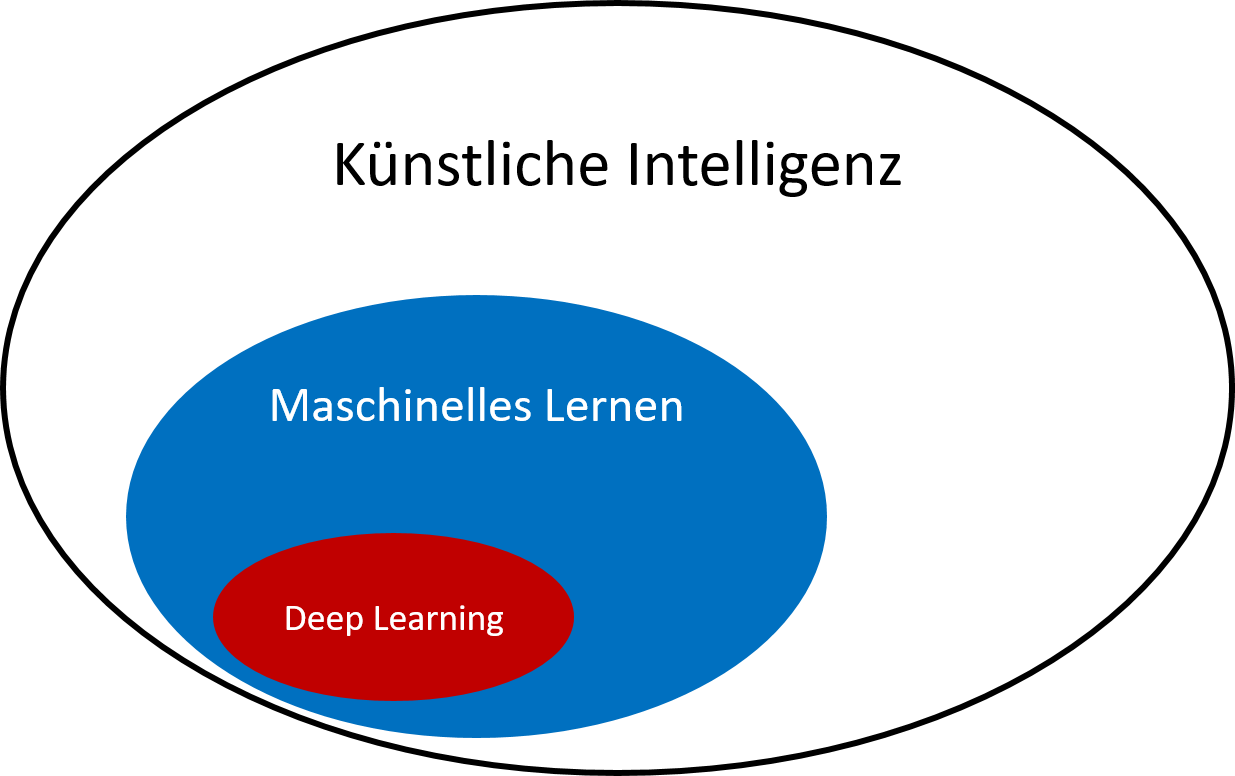
\includegraphics[scale=0.2]{images/MLInAI}
\cite{MLEinordnung}
\end{frame}

\begin{frame}{Einordnung von maschinellem Lernen}
\begin{itemize}
\item{Künstliche Intelligenz: Jede Technik, die es einem Computer ermöglicht auf seine Umgebung zu reagieren.}
\item{Maschinelles Lernen: Teilbereich der Künstlichen Intelligenz. Jede Technik, die mit statistischen Methoden dem Computer ermöglicht durch Erfahrung seine Funktion zu verbessern.}
\item{Deep Learning: Teilbereich von Maschinellem Lernen. Nutzt künsliche neuronale Netze mit zahlreichen Zwischenlagen.}
\end{itemize}
\end{frame}

\begin{frame}{Anwendungen}
\begin{itemize}
\item{Gesichtserkennung}
\item{Umwandlung von gesprochener Sprache zu Text}
\item{Handschrifterkennung}
\item{Autonomes Fahren}
\item{Maschinelle Übersetzungen}
\end{itemize}
\end{frame}

\section{Künstliche neuronale Netze}

\begin{frame}{Künstliche neuronale Netze}
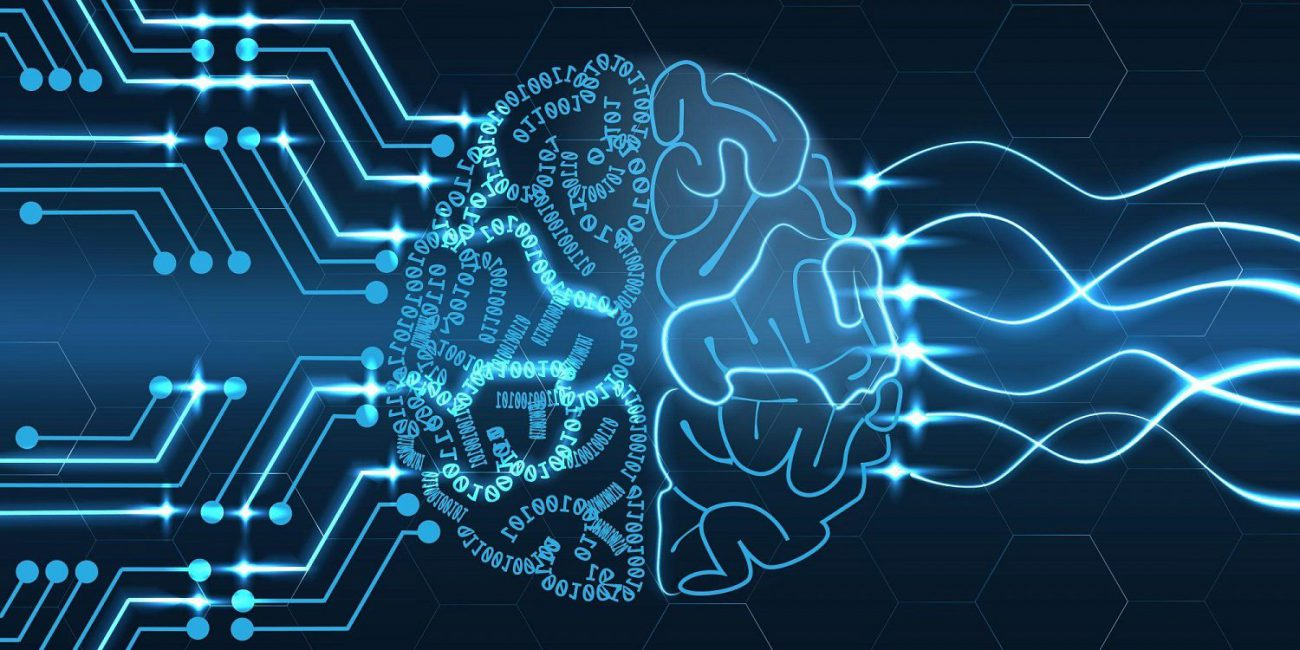
\includegraphics[scale=0.25]{images/BrainNN.jpg}
\cite{BrainNN}
\end{frame}

\begin{frame}{Künstliche Neuronale Netze}
Ziele:
\begin{itemize}
\item{Klassifizieren}
\item{Zusammenhänge erkennen}
\end{itemize}
\end{frame}

%\begin{frame}{Perceptron}
%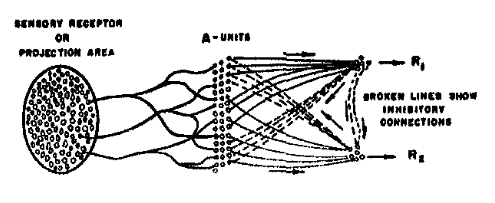
\includegraphics{images/perceptron.png}
%\cite{rosenblatt1958perceptron}
%\end{frame}

\begin{frame}{Fully connected neural network}
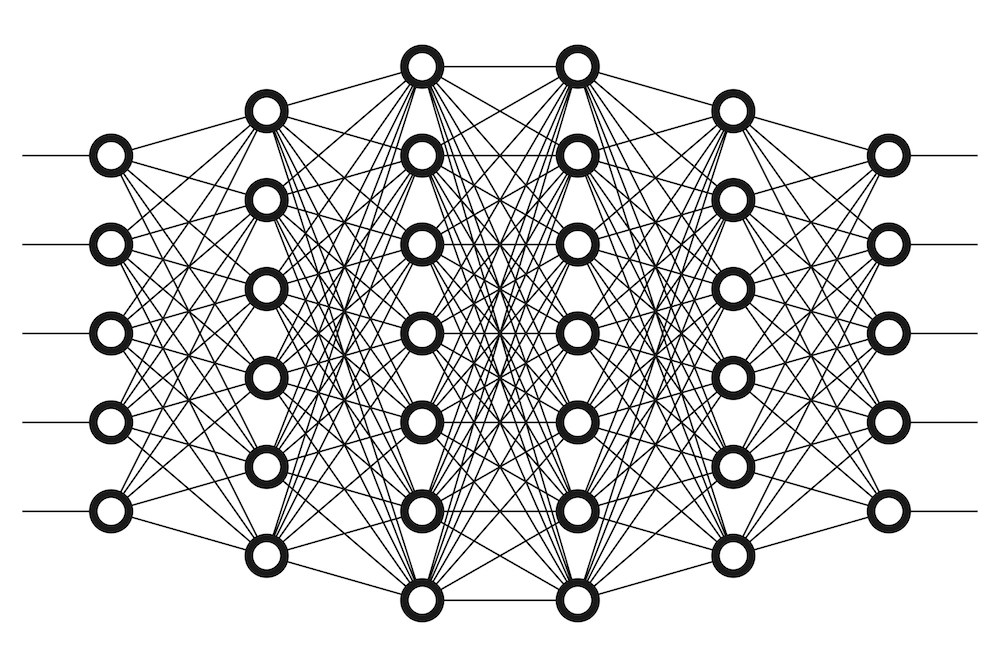
\includegraphics[scale=0.4]{images/DeepNeuralNetwork.jpg}
\cite{Raicea2018Jun}
\end{frame}

\subsection{Propagierungsfunktion}

\begin{frame}{Propagierungsfunktion}
\begin{itemize}
\item{Jede verbindung zwischen zwei Neuronen besitzt eine Gewichtung (\textit{Engl: weigth}) w}
\end{itemize}
\end{frame}

\begin{frame}{Propagierungsfunktion}
Die \textit{Propagierungsfunktion} berechnet den Input $p_j^{l}(t)$ des Neurons j anhand der Outputs $o_i(t)$ der Neuronen in der vorangehenden Lage $l$.
\begin{equation}
p_j^{(l+1)}(t) = \sum_{i}^{} o_i^{(l)}(t) w_{ij}^{(l)}
\end{equation}
\end{frame}

\subsection{Trainieren eines künstlichen neuronalen Netzes}

\begin{frame}{Trainieren eines künstlichen neuronalen Netzes}
Anpassung der Gewichte:
\begin{equation}
w_{ij}^{neu} = w_{ij}^{alt} + \Delta w_{ij},\ mit
\end{equation}
$w_{ij}^{neu}$ der neue Wert des Gewichts der Verbindung zwischen Neuronen i und j\\
$w_{ij}^{alt}$ der alte Wert des Gewichts	der Verbindung zwischen Neuronen i und j	\\
$\Delta w_{ij}$ die Änderung des Gewichts der Verbindung zwischen Neuronen i und j
\end{frame}

\begin{frame}{Elman recurrent neural network}
\begin{center}
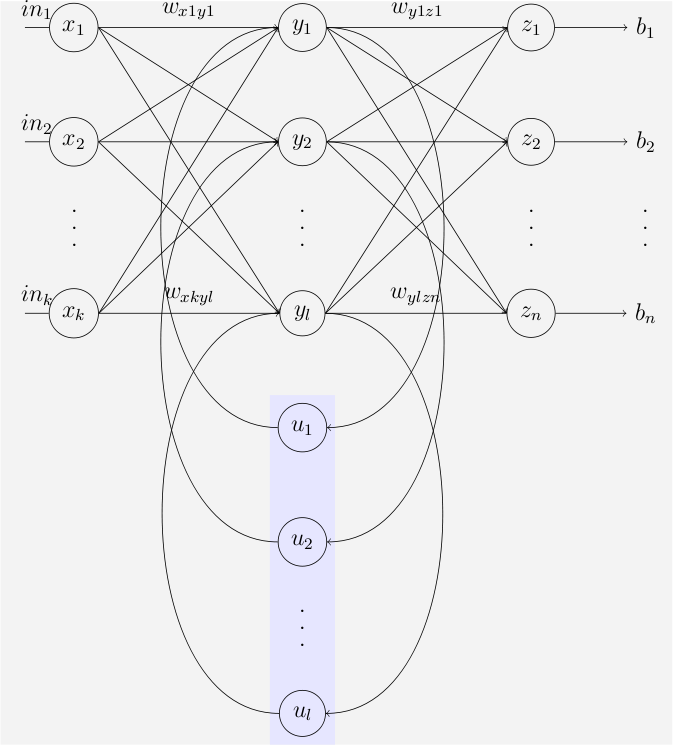
\includegraphics[scale=0.25]{images/Elman_RNN.png}
\cite{Elman}
\end{center}
\end{frame}

\subsection{Limitationen von neuronalen Netzen}

\begin{frame}{Limitationen von neuronalen Netzen}
\begin{itemize}
\item{Rechenintensiv}
\item{Es werden massive Datenmengen benötigt}
\item{Es kann in der Regel nicht verstanden werden weshalb eine Entscheidung getroffen wird}
\end{itemize}
\end{frame}

\section{Maschinelle Übersetzungen}

\begin{frame}{Maschinelle Übersetzungen}
\begin{itemize}
\item{Google, Microsoft und Yandex nutzen alle neural machine translation}
\end{itemize}
\end{frame}

\begin{frame}{Google neural machine translation}
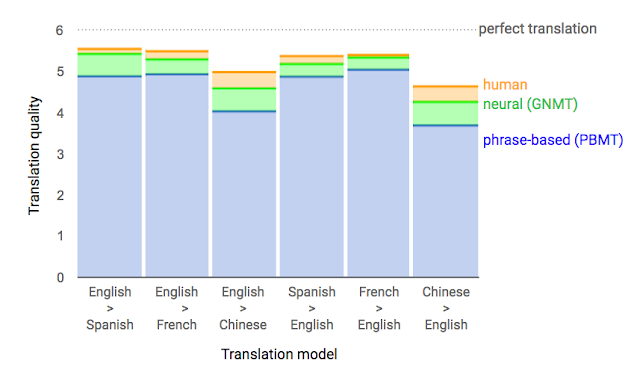
\includegraphics[scale=0.5]{images/MTGoogle.png}
\cite{googleaiblog_2016}
\end{frame}

\section{Kuriositäten}

\begin{frame}{Kuriositäten}
\begin{itemize}
\item{Facebook Chatbots erfinden ihre eigene Sprache}
\item{Google neural machine nutzt eine neue Zwischensprache}
\end{itemize}
\end{frame}

\begin{frame}{Facebook Chatbots}
\begin{center}
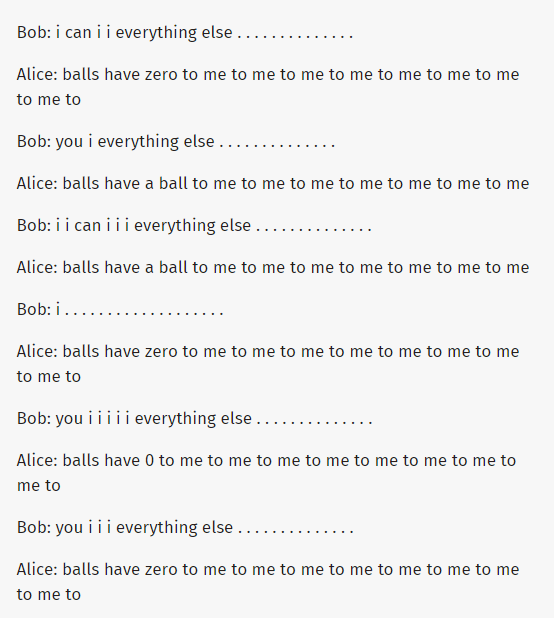
\includegraphics[scale=0.4]{images/FacebookChatbots.png}
\cite{wilson_2018}
\end{center}
\end{frame}

\begin{frame}{Google neural machine translation}
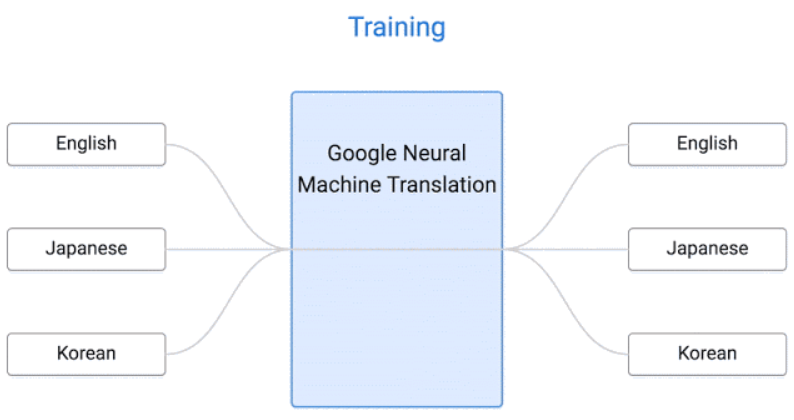
\includegraphics[scale=0.7]{images/GNTM.png}
\cite{Korbut2018Jun}
\end{frame}

\section{Bewertung}

\begin{frame}{Bewertung}
\begin{itemize}
\item{Mehr als nur Hype}
\item{Gefahren und Limitationen}
\end{itemize}
\end{frame}

\begin{frame}{Vielen Dank}
\begin{center}
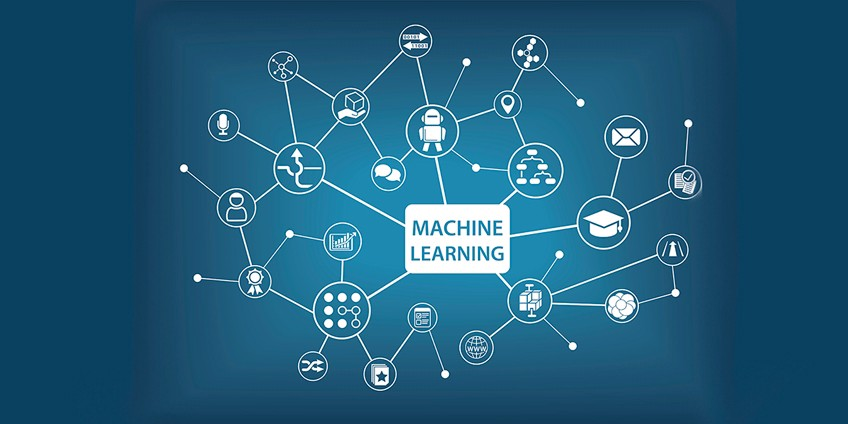
\includegraphics[scale=0.35]{images/VielenDank.jpeg}
\cite{Dwivedi2018Jun}
\end{center}
\end{frame}
\appendix
\beginbackup

\begin{frame}[allowframebreaks]{References}
\printbibliography
\end{frame}

\backupend

\end{document}
